\section{The Onset of Color Transparency}
The signature of the onset of CT is a rise in $T$ with $Q^2$ above some
threshold $Q^2_0$.
Previous measurements of T in ${}^{12}C(e,e'p)$ at SLAC, MIT-Bates, and JLab
for momentum transfers between $Q^2=0.6$ and
\SI{8.1}{\giga\electronvolt\squared} have been consistent with the predictions
of the Glauber model.

The model presented by Frankfurt et al.~\cite{Frankfurt_1995_PRC} starts by
calculating the amplitude $\mathcal{M}_{h}^{\gamma^*A}$ for quasielastic
scattering of a proton from a fixed shell $h$ in a nucleus.
This amplitude includes the effects of short range nucleon-nucleon
correlations, both between the ejected proton and remainder nucleons in the
recoil nucleus as well as between the remainder nucleons.
Using the distorted wave impulse approximation (DWIA), they derive an
expression for nuclear transparency whose behavior is dependent on the form of
nucleon-nucleon interactions.
These interactions are parameterized by profile functions $\Gamma(\vec{b})$
that are a function of impact parameter $\vec{b}$.
They compare two choices of profile function--one which corresponds to the
absence of CT and one which includes a model of CT in which~\cite{Farrar_1988}
the PLC grows to the full size of a proton over a length $l_h$, the hadron
formation length.


The model presented by Cosyn et al.~\cite{Cosyn_2008,Cosyn_2006} uses a
relativistic multiple scattering Glauber approximation~\cite{Ryckebusch_2003}
that accounts for final state interactions by applying a phase to the ejected
proton's wavefunction.
This phase is determined by a profile function $\Gamma(\vec{b})$ that
parameterizes nucleon-nucleon scattering.
As in the other model, this profile function is modified to include CT effects
Short range correlations are implemented by means of an effective nucleon
density~\cite{Frankel_1994} that enters into the calculation of the Glauber
phase.


To include CT effects, both models replace the total cross section
$\sigma_{tot}$ with an effective cross section $\sigma_{eff}$
based on a quantum diffusion model~\cite{Farrar_1988}
that accounts for reduced interaction between the prehadron and nuclear matter
over a hadron formation length $l_h$,
\begin{equation}
    \sigma_{eff} = \sigma_{tot}
    \left\{
        \left[\frac{z}{l_h} +
               \frac{\left\langle n^{2} k_{t}^{2}\right\rangle}{t} \left(1-\left(\frac{z}{l_h}\right)\right)
        \right]
        \theta\left(l_h-z\right) +
        \theta\left(z-l_h\right)
    \right\}
\end{equation}
In this expression,
$n$ is the number of valence quarks (2 for mesons, 3 for baryons),
$k_t \sim \SI{1}{\giga\electronvolt\squared}/Q^2$
is the average transverse momentum of a quark inside a hadron,
$z$ is the distance the object has traveled since its creation,
and
$l_h=2p/\Delta M^2$ is the hadronic formation length.
This length depends on
the momentum $p$ of the outgoing hadron
and
the mass squared difference between the prehadron and outgoing hadron state.
Frankfurt et al. use $\Delta M^2 = \SI{0.7}{\giga\electronvolt\squared}$
for protons, while
Cosyn et al. use $\Delta M^2 = \SI{1.0}{\giga\electronvolt\squared}$.

\subsection{Frankfurt et al.}

% Frankfurt et al. derive an modified nuclear density $\tilde{\rho}(r)$ that
% takes nucleon correlations into account based on single nucleon density
% functions $\rho(r)$ and two-body correlation functions $g_h(r,r')$,
% \begin{equation}
%     \tilde{\rho}(r)
%         = (A-1) \rho(r)
%           \left[
%                1 + C_h(r_1,r) - \frac{A-1}{2} \int_{z_1} \Gamma(b_1-b')g_h(r,r')\rho(r')d^3r'
%           \right]
% \end{equation}
% Here, $C_h(i,j)$ are two-nucleon correlation factors that are functions of the
% distance $r_{ij}=|\vec{r}_j-\vec{r}_i|$ between nucleons $i$ and
% $j$~\cite{Weise_1972}.
% The single nucleon wave functions $\phi_h(r)$ are the overlap integral between
% wave functions of the $A$-body ground state wave function and the $(A-1)$-body
% recoil nucleus.
% Their normalization requires $\int|\phi_h(r)|d^3r=1$ and
% $\rho(r) = \sum_h \omega_h^2 \left| \phi_h(r) \right|$ where $\omega_h$ is the
% occupation probability of the orbital $h$.

% \begin{equation}
%     \mathcal{M}_{h}^{\gamma^*A} = \int d^3 r_1 \omega_h \phi_h\left(r_{1}\right)
%                                   \hat{O}^{\mathrm{em}}\left(Q^{2}\right)
%                                   e^{-i \vec{p}_p \cdot \vec{r}_1}
%                                   \exp{- \int_{z_{1}}
%                                   \Gamma\left(b_{1}-b\right) \tilde{\rho}(r) d^3 r}
% \end{equation}

In the DWIA, the cross section can be written
\begin{equation}
    \frac{d^6\sigma}{dE'_{e} d\Omega'_{e} d^3p'_{p}} = p'_p E'_p \sigma_{eN} S(\vec{p}_p, E_M, \vec{p'}_p)
\end{equation}
where $\sigma_{eN}$ is the cross section for an electron scattering from a
bound nucleon and $S(\vec{p}_p, E_M, \vec{p'}_p)$ is the distorted
spectral function.
For a fixed shell $h$ the spectral function can be written~\cite{Frullani_1984},
\begin{equation}
    S(\vec{p}_p, E_M, \vec{p'}_p) = n_h(E_m) |\Phi_h(\vec{p}_p, \vec{p'}_p)|^2
\end{equation}
where $\Phi_h(\vec{p}_p, \vec{p'}_p)$ is the distorted momentum distribution for
nucleons in the $h$ shell
and
$n_h(E_m)$ (proporitonal to the shell's occupation probability) characterizes
the strength of the shell.
Frankfurt et al. derive the following expression for the momentum distribution
by expressing the ground state $A$-body wave function and $(A-1)$-body density
matrix in terms of two-nucleon correlation functions
\begin{equation}
    \left| \Phi_h(\vec{p}_p, \vec{p'}_p)\right|^2
        = \left|
            \int d^3 r_1 \Psi_h(r_1) e^{-i \vec{p}_p \cdot \vec{r}_1}
            \exp{\left\{- \int_{z_{1}} \Gamma\left(\vec{b}_1-\vec{b}\right) \tilde{\rho}(r) d^3 r\right\}}
          \right|
\end{equation}

The profile function $\Gamma(\vec{b})$ takes the form
\begin{equation}
    \Gamma(\vec{b}) = \frac{1}{2\pi i k}
                  \int e^{i\vec{k}_t \cdot \vec{b}} f(\vec{k}_t) d^2k_t
\end{equation}
where the nucleon-nucleon scattering amplitude with CT effects is
\begin{equation}
    f_{CT}(k_t, z, Q^2) = i\frac{k}{4\pi} \sigma_{eff}(z,Q^2) e^{Bt/2}
                          \frac{G_N\left( t \sigma_{eff}(z,Q^2)/\sigma_{eff} \right)}
                               {G_N\left( t \right)}
\end{equation}
and the amplitude without CT effects is
\begin{equation}
    f(k_t) = \left(\frac{k_t}{4\pi}\right)^2
             \sigma_{tot}^2
             (1+\epsilon^2) e^{-Bt}
\end{equation}
%All prameters are taken from their refs 29-31
where
$\epsilon$ is the ratio of the scattering amplitude's real and imaginary parts
and
$B$ is a slope parameter.

The nuclear transparency for the $h$ shell is the ratio of the distorted
momentum distributions from the DWIA and PWIA,
\begin{equation}
    T_h = \left(\frac{\sigma^{exp}}{\sigma^{PWIA}}\right)
        = \frac{|\Phi^{DWIA}_h(p_p,p'_p)|^2}
               {|\Phi^{PWIA}_h(p_p)|^2}
\end{equation}

Transparency predictions for ${}^{12}C(e,e'p)$ scattering from the $s$ shell,
with and without CT, are shown in Fig~\ref{fig:frankfurt_transparency}.

% The ground state wavefunctions Frankfurt et al. use are calculated in the
% Skyrme-Hartree-Fock model with correlated interactions~\cite{Reinhard_1991}.

\begin{figure}[h]
    \centering
    \begin{subfigure}[b]{0.45\textwidth}
        \centering
        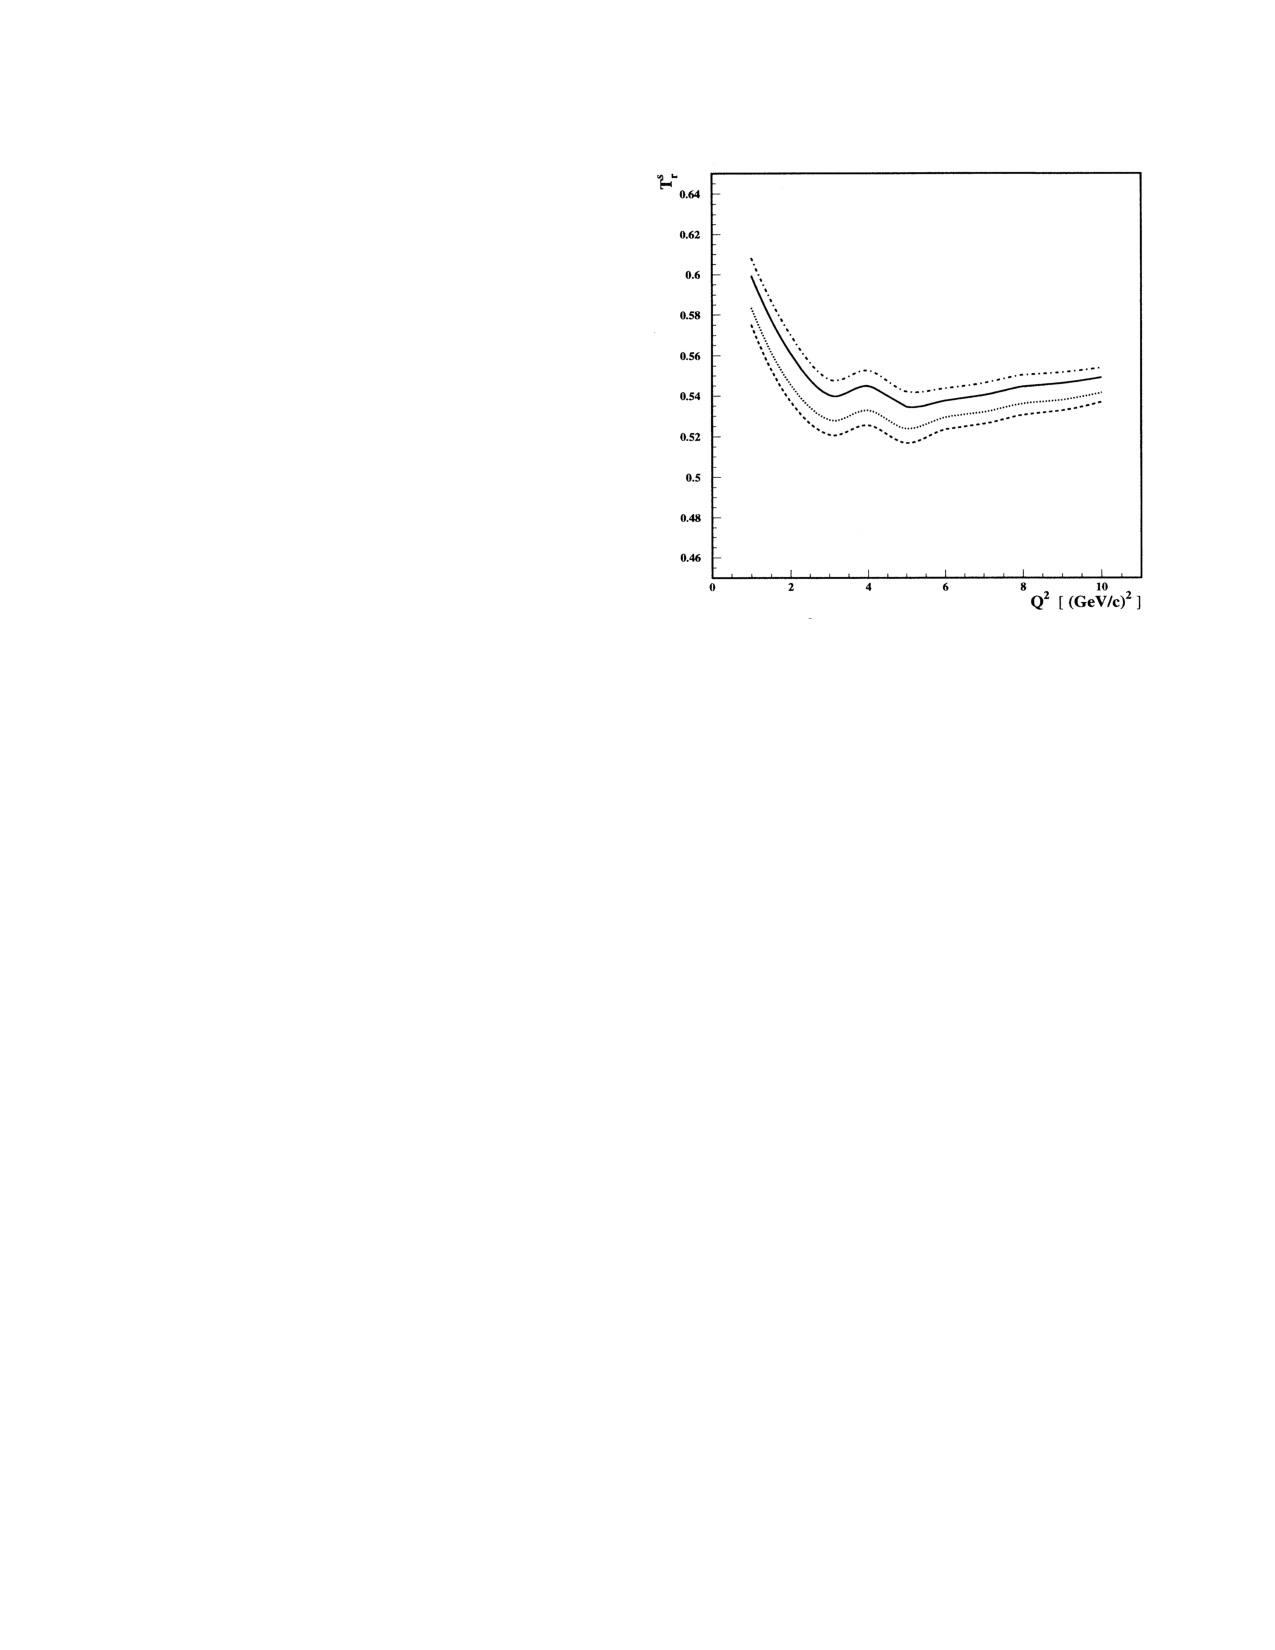
\includegraphics[width=\textwidth]{chap1/frankfurt_transparency_without_CT.pdf}
        % \caption{X plane}
        \label{fig:frankfurt_transparency_without_CT}
    \end{subfigure}
    % \hfill
    \begin{subfigure}[b]{0.45\textwidth}
        \centering
        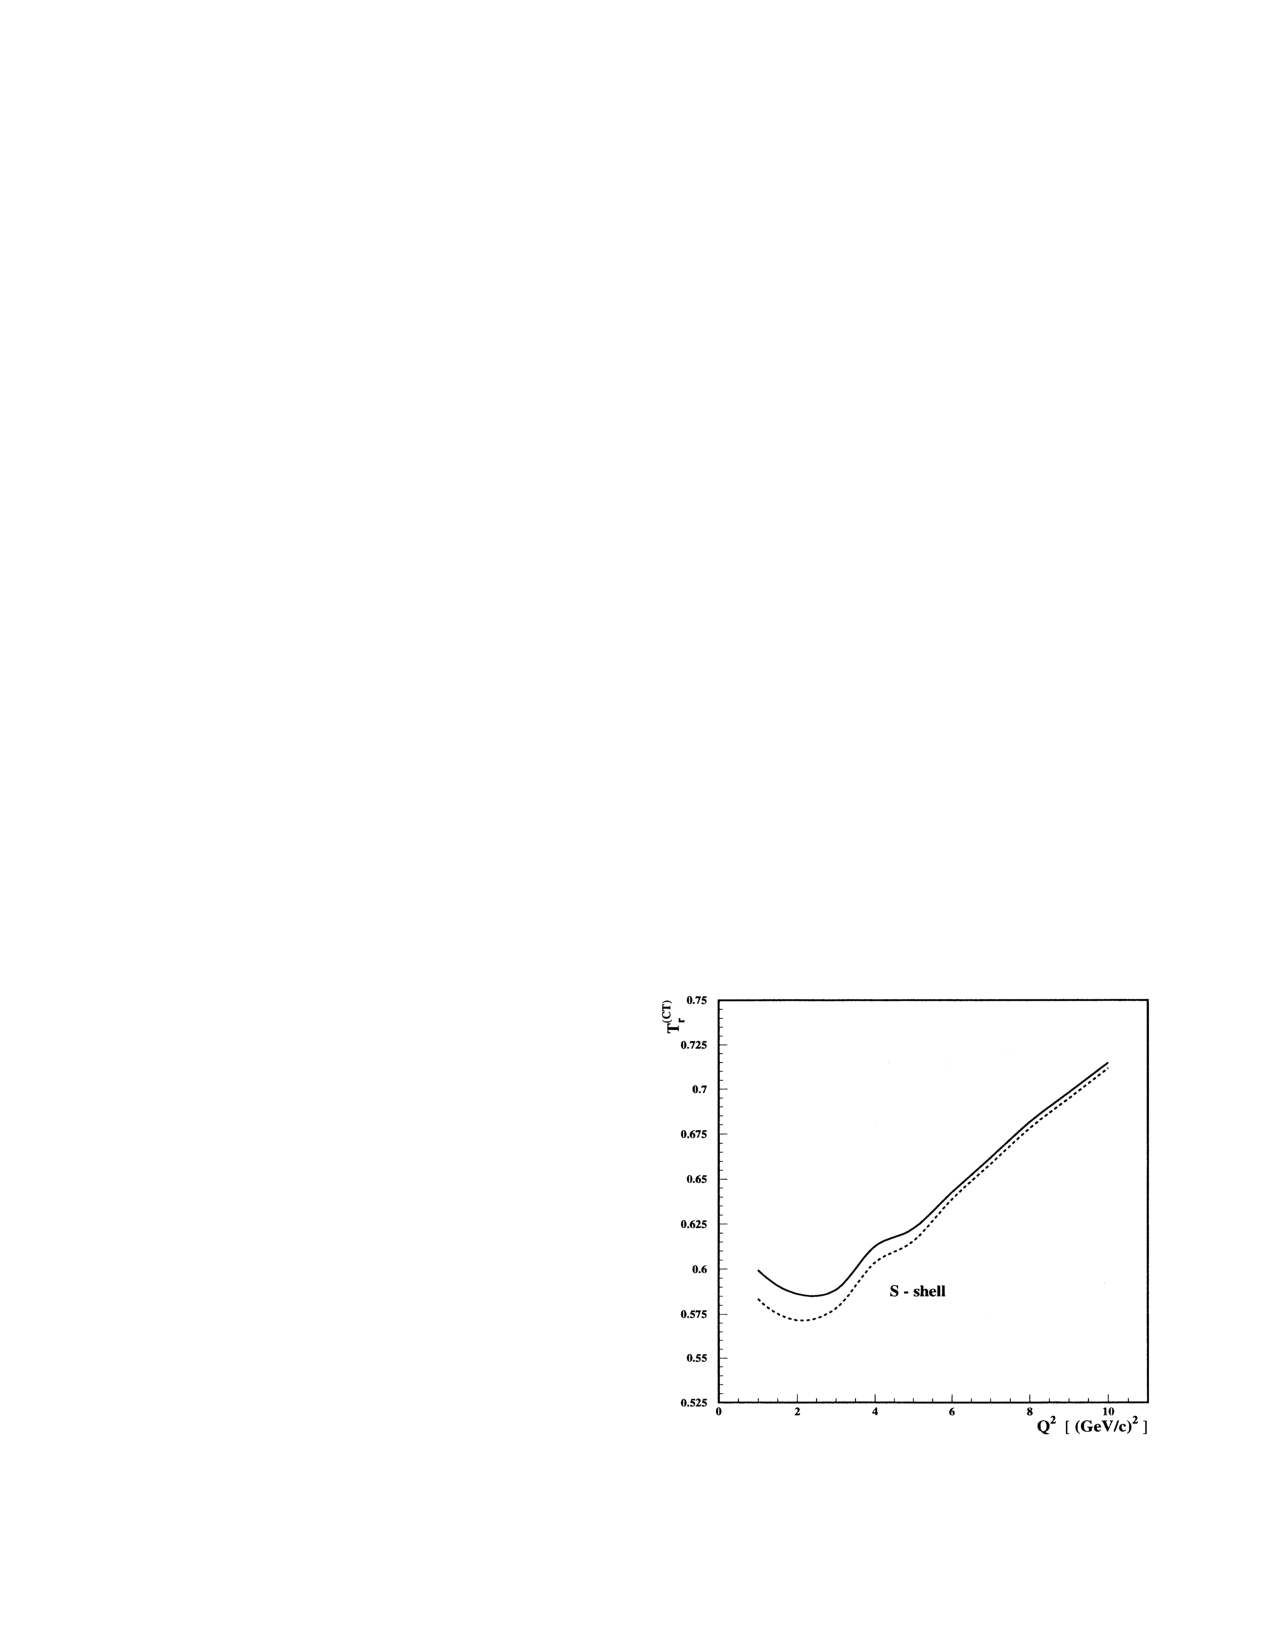
\includegraphics[width=\textwidth]{chap1/frankfurt_transparency_with_CT.pdf}
        % \caption{U plane}
        \label{fig:frankfurt_transparency_with_CT}
    \end{subfigure}
    \caption{Transparency calculations for ${}^{12}C(e,e'p)$ based on a model
             that accounts for nucleon correlations and proton knock-out from
             particular nuclear shells~\cite{Frankfurt_1995_PRC}.
             The figure on the left is for a model that does not include CT.
             The dotted line is the calculation without correlation effects;
             the dashed line, with the effects of correlation between undetected nucleons;
             the dash-dotted line, with the effects of correlation between knocked-out proton and undetected nucleons;
             and solid line, with over-all correlation effects.
             The figure on the right includes CT.
             The dashed line is the calculation without correlation effects;
             the solid line, with corrleation effects.
             The rise in transparency with $Q^2$ is the characteristic
             signature of the onset of CT.
             Note that the effect of nucleon correlations on the CT model is
             a correction of a few percent.
             }
    \label{fig:frankfurt_transparency}
\end{figure}



\subsection{Cosyn et al.}

The model of Cosyn et al. derives eikonal approximation of equation~\ref{eqn:eikonal_approximation}.
After rescattering, the outgoing wavefunction $\psi_{out}$ picks up a complex
phase $\chi(\vec{r})$.
\begin{equation}
    \psi_{out}(\vec{r}) = e^{i\chi(\vec{r})} \psi_{in}(\vec{r})
\end{equation}

This phase can be parameterized as a function of impact parameter $\vec{b}$,
momentum transfer $Q^2$, etc. by a profile function $\Gamma(\vec{b})$.
For a single rescattering,
\begin{equation}
    \psi_{out}(\vec{r}) = (1-\Gamma(\vec{b})) \psi_{in}(\vec{r})
\end{equation}

Every spectator nucleon in the recoil nucleus lying in the forward path of the
ejected proton contributes to the total phase.
Let $\vec{r}$ be the point at which the ejected proton absorbs the virtual
photon.
The total phase shift for $A$ nucleons is a product
\begin{equation}
    e^{i\chi(\vec{r})} = \prod_{j=2}^{A} \left(1-\Gamma(\vec{b}_j)\theta(z_j-z)\right)
\end{equation}

The profile function for a hadron $h$ scattering from a nucleon $N$ is
determined by
the interaction cross section $\sigma^{hN}_{tot}$,
the ratio $\epsilon_{hN}$ of the scattering amplitude's real and imaginary parts,
and slope parameter $\beta_{hN}$,
all of which are momentum-dependent.
These parameters can be estimated by interpolating data from the Particle Data
Group.
\begin{equation}
    \Gamma(\vec{b}) =
        \frac{\sigma^{hN}_{tot}(1-i\epsilon_{hN})}
             {4\pi\beta_{hN}^2}
        \exp{-\frac{\vec{b}^2}{2\beta_{hN}^2}}
\end{equation}

The slope parameter $\beta_{hN}$ can be estimated using
the elastic $\sigma^{hN}_{el}$ and total $\sigma^{hN}_{tot}$ cross sections
in the following
approximation~\cite{Ryckebusch_2003}
\begin{equation}
    \beta_{p N}^{2} \approx
            \frac{(\sigma^{hN}_{tot})^{2} (\epsilon_{hN}^{2}+1)}
                 {16 \pi \sigma^{hN}_{el}}
\end{equation}

